\section{Competitive Ratio General $k$}
\label{app:general_k_proof}
We now prove our main result for the competitive ratio of \algoname \ for $k \geq 2$. The theorem statement is reproduced here for convenience.  
\begin{reptheorem}{thm:general_k_theorem1}
The competitive ratio of \algoname\ for $k \geq 2$ and where $t = \alpha n$ can asymptotically be lower bounded by 
\begin{equation}
    C_k >  \max_{\alpha \in [0,1]}  {\alpha}^k \left(\sum_{m = 0}^{k - 1} a_m \ln^m (\alpha)\right) - \alpha a_0
    \hspace{0.15cm }where  \hspace{0.15cm }
    a_m = \left(\frac{\frac{k^k}{(k-1)^{k-m}} - k^m}{m!}\right)(-1)^{m+1}
    \, .
\end{equation}

\end{reptheorem}
\begin{figure}[ht]
    \centering
    %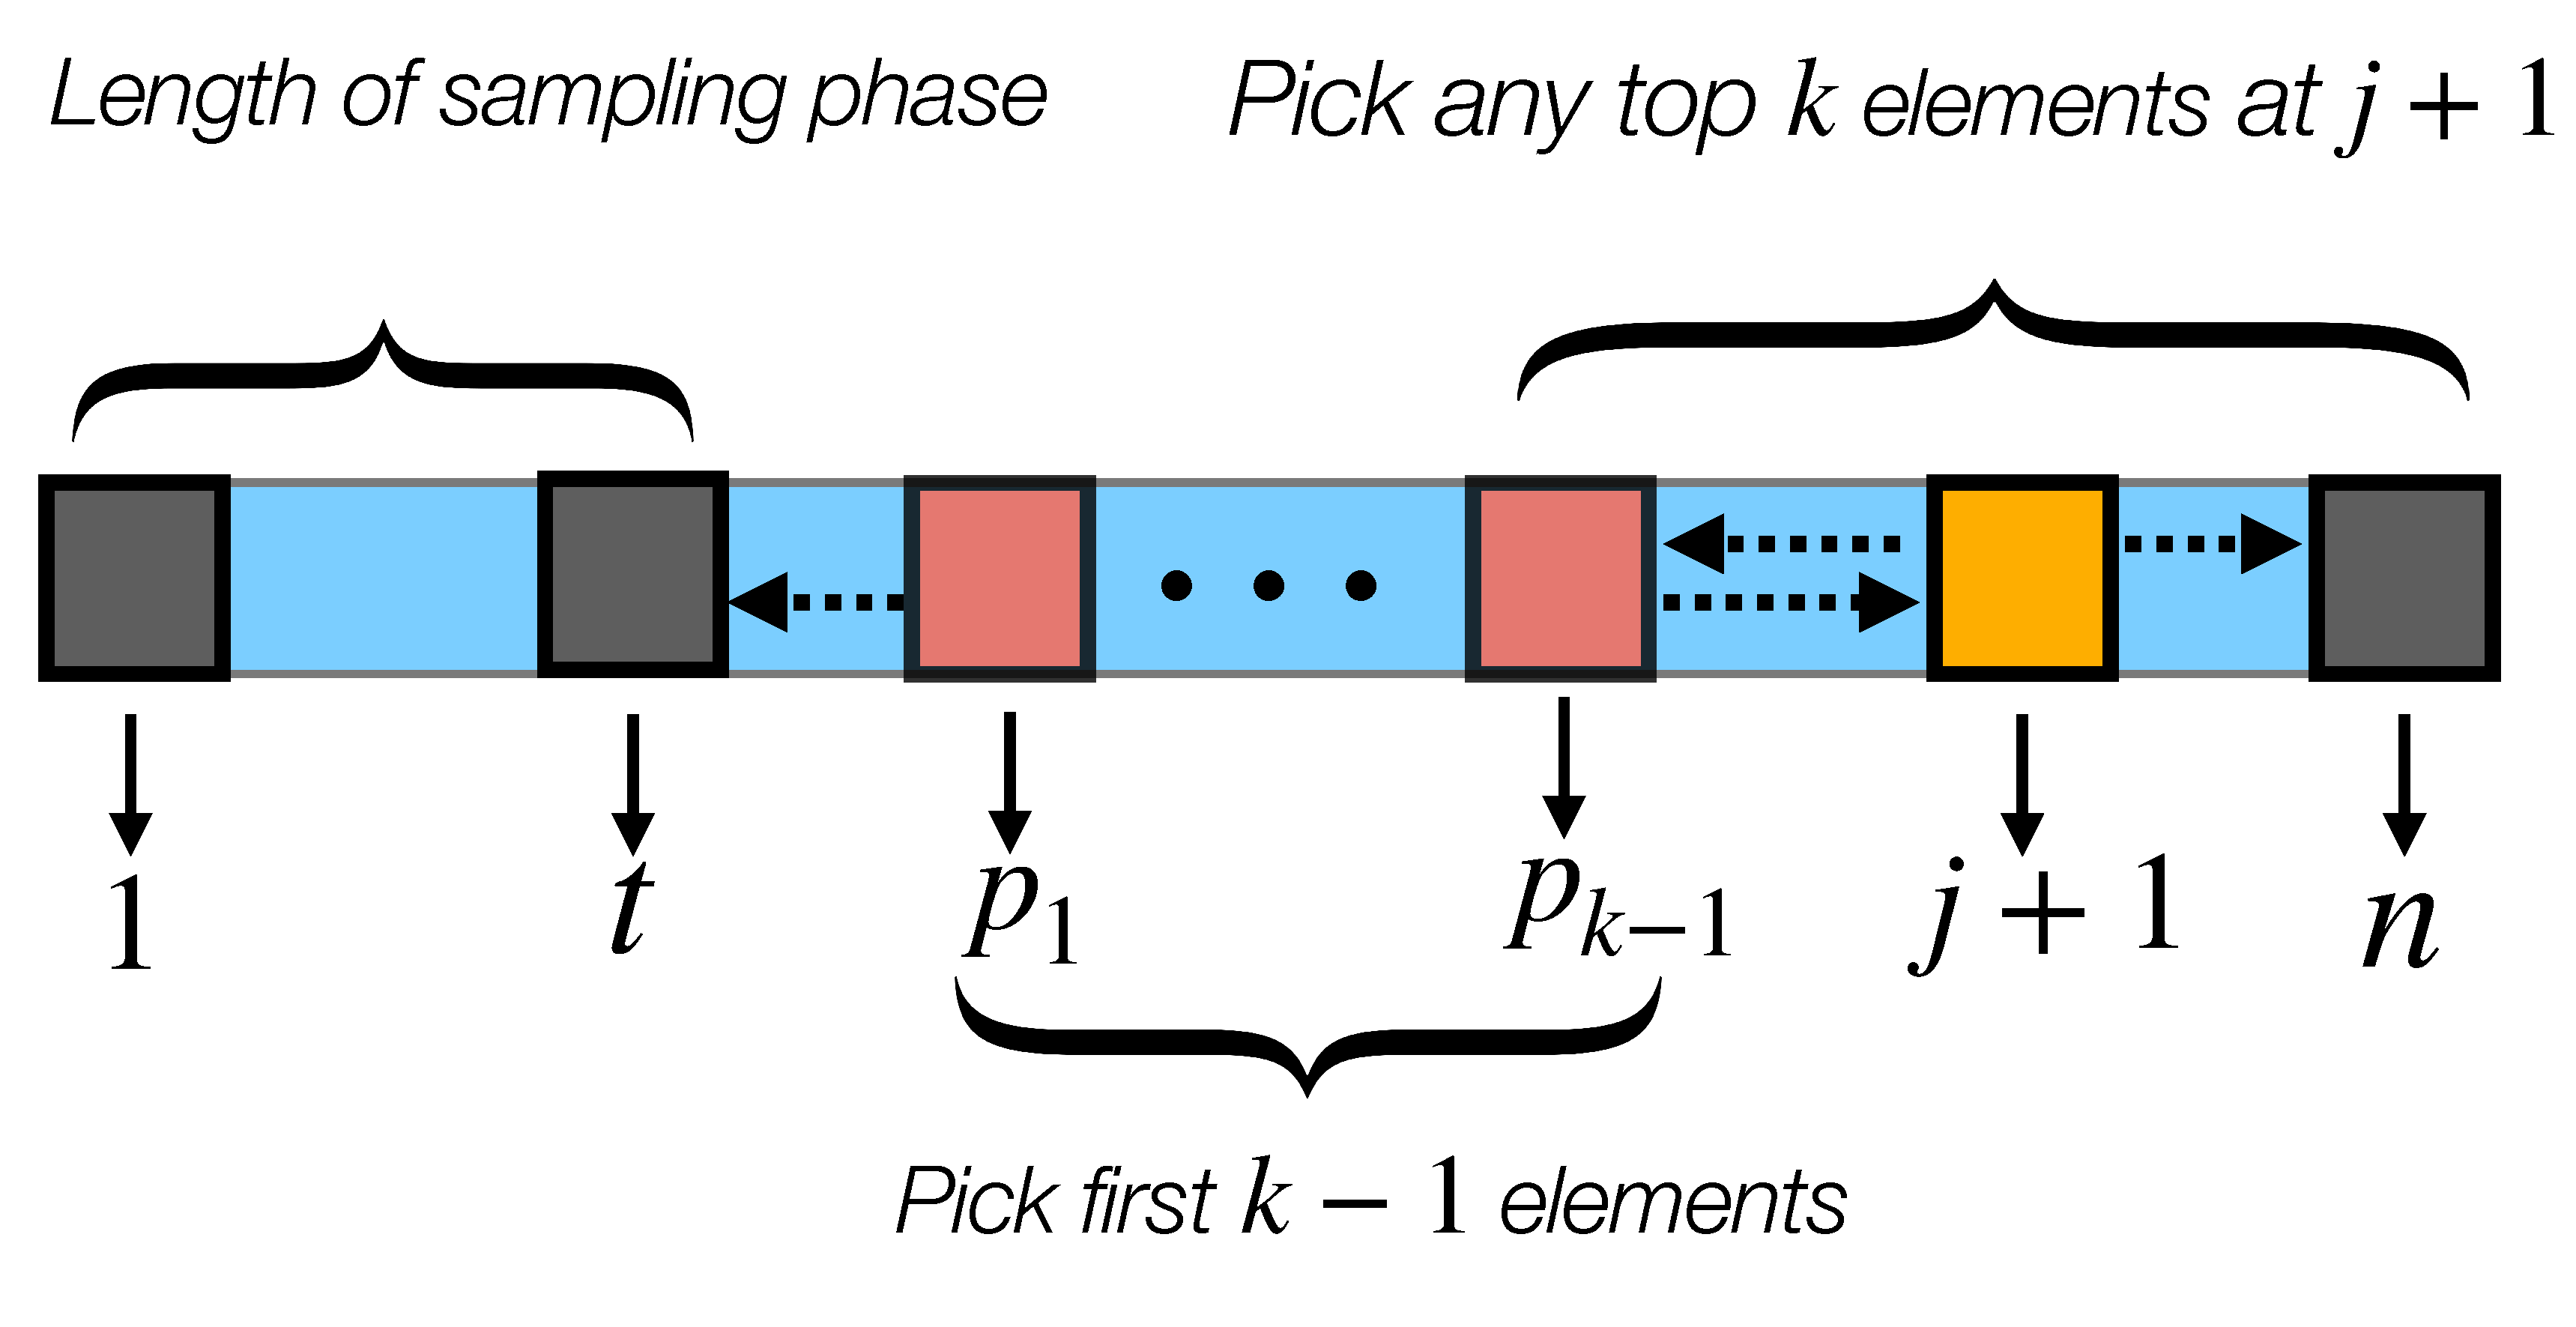
\includegraphics[width=0.50\linewidth]{Figures/virtual_plus_general_k.pdf}
    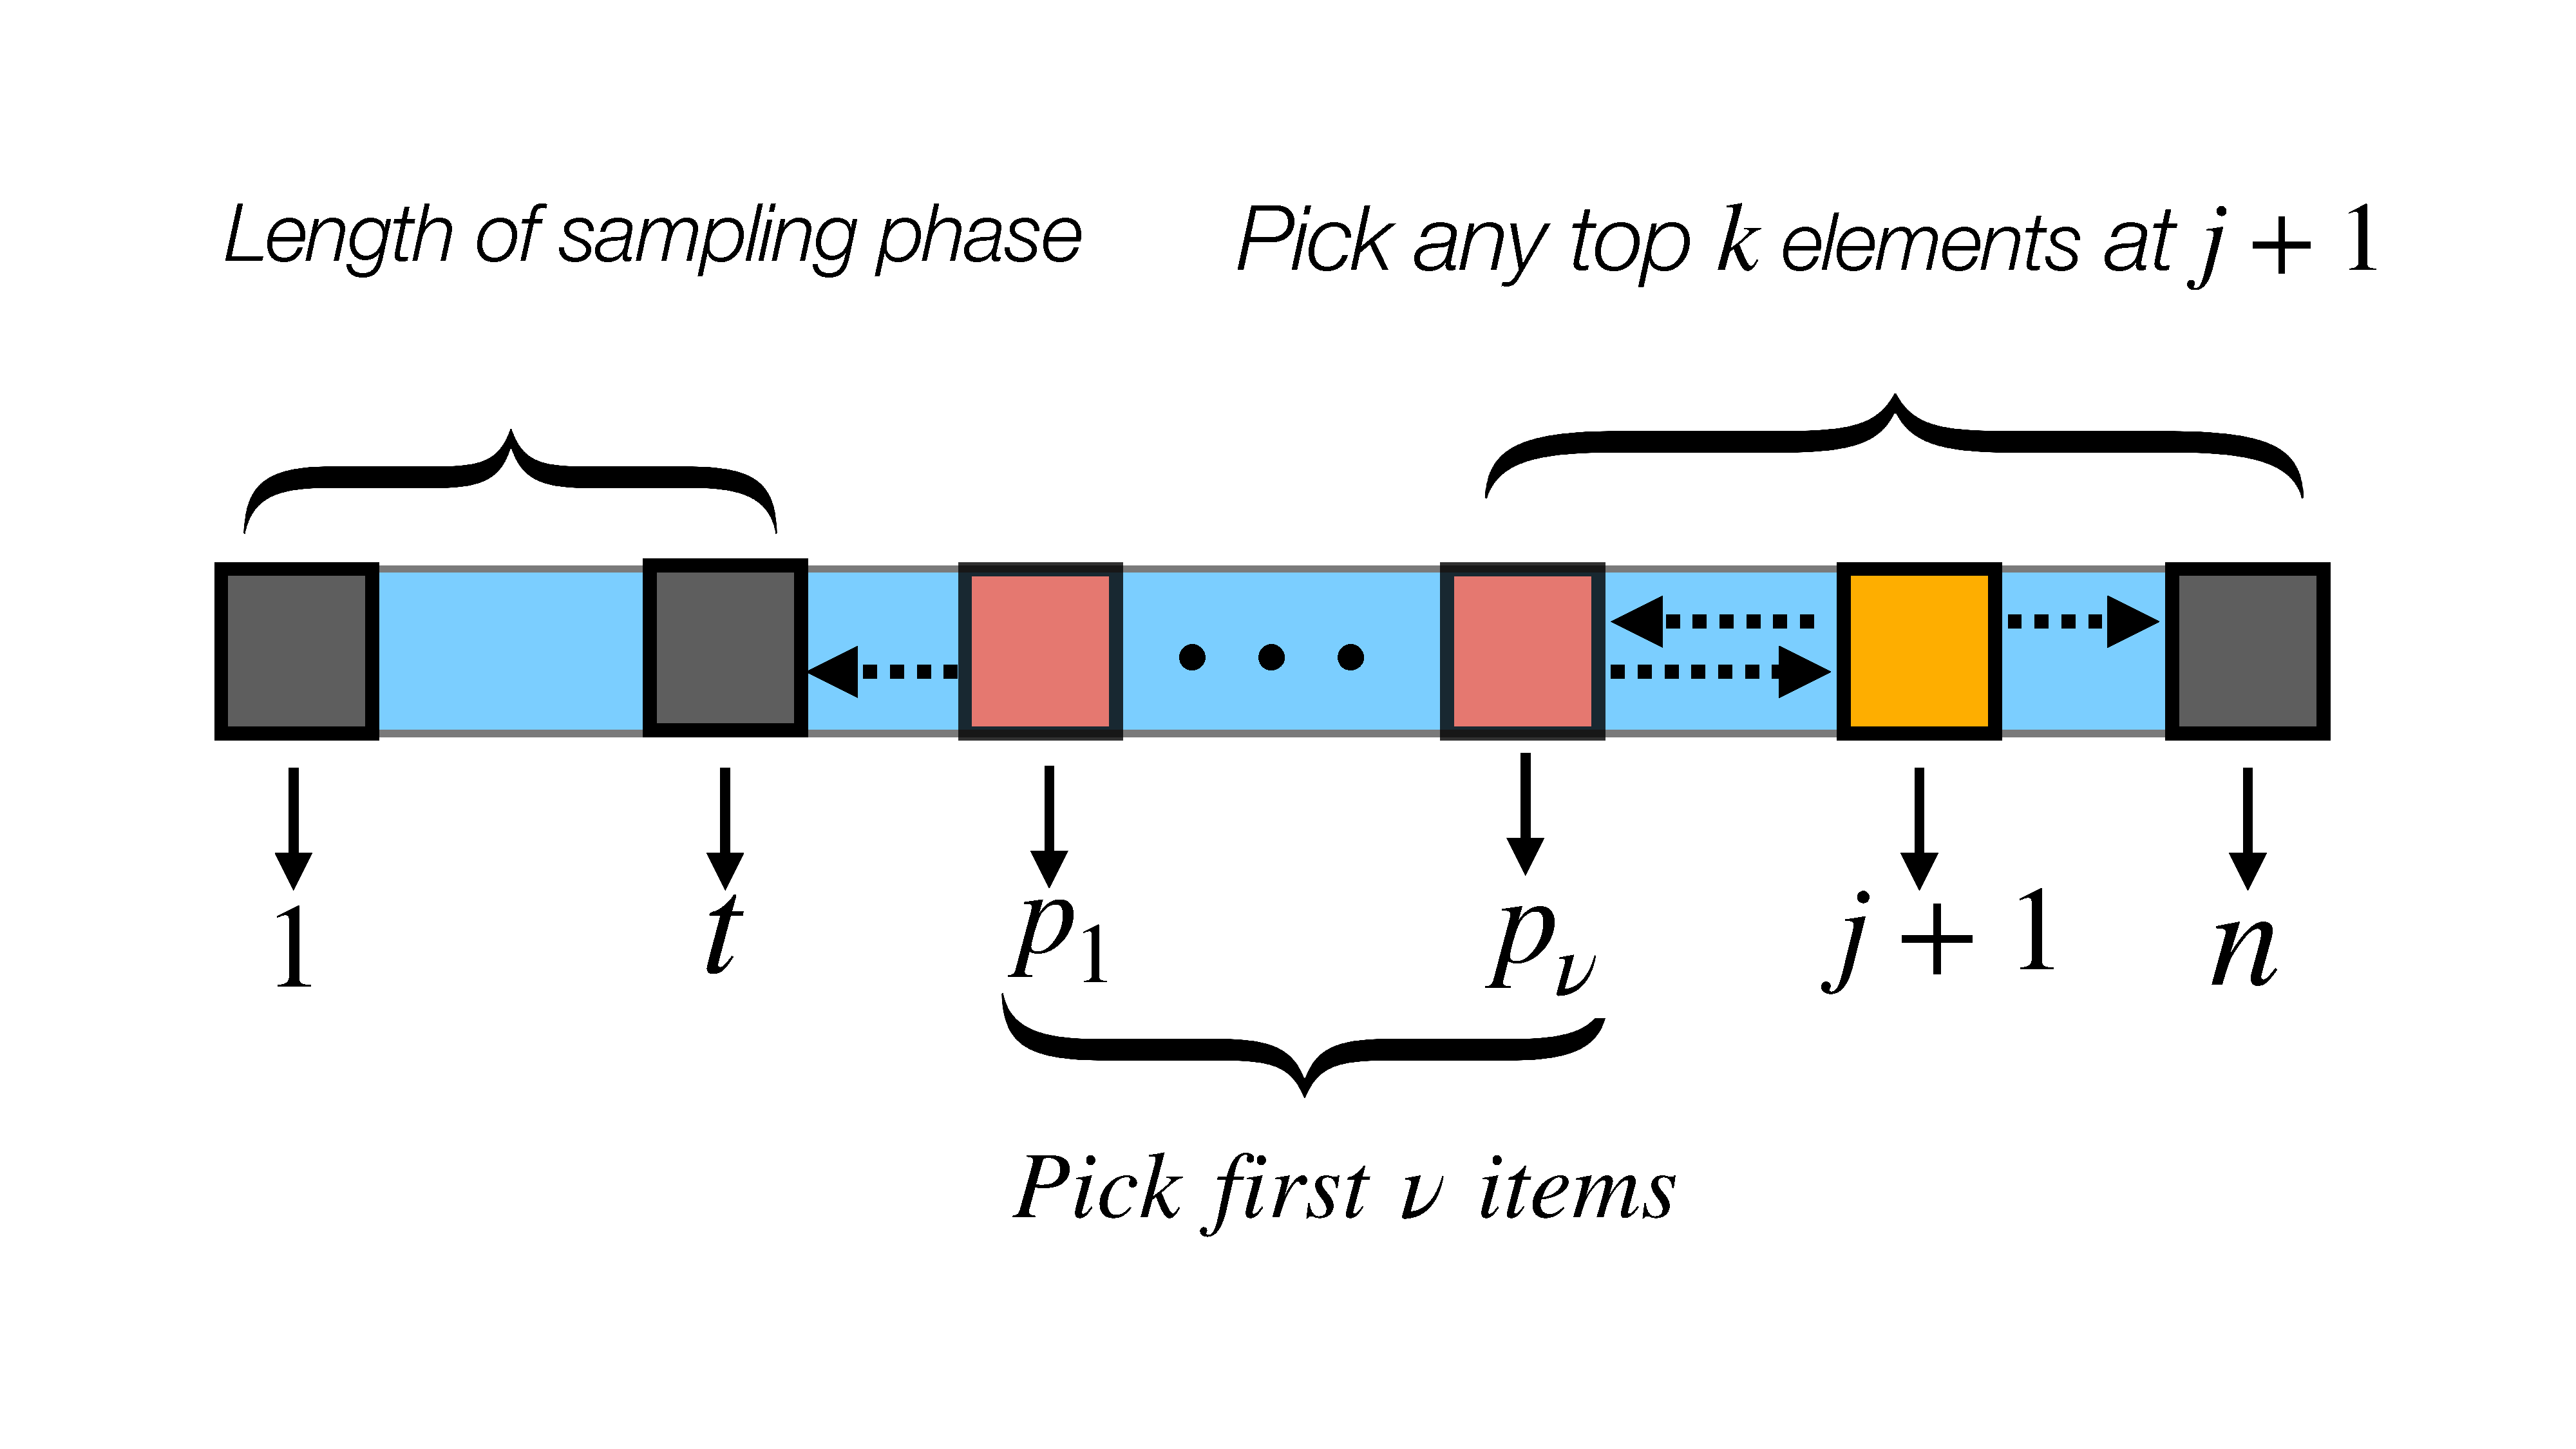
\includegraphics[width=1.0\linewidth]{Figures/general_k.pdf}
    %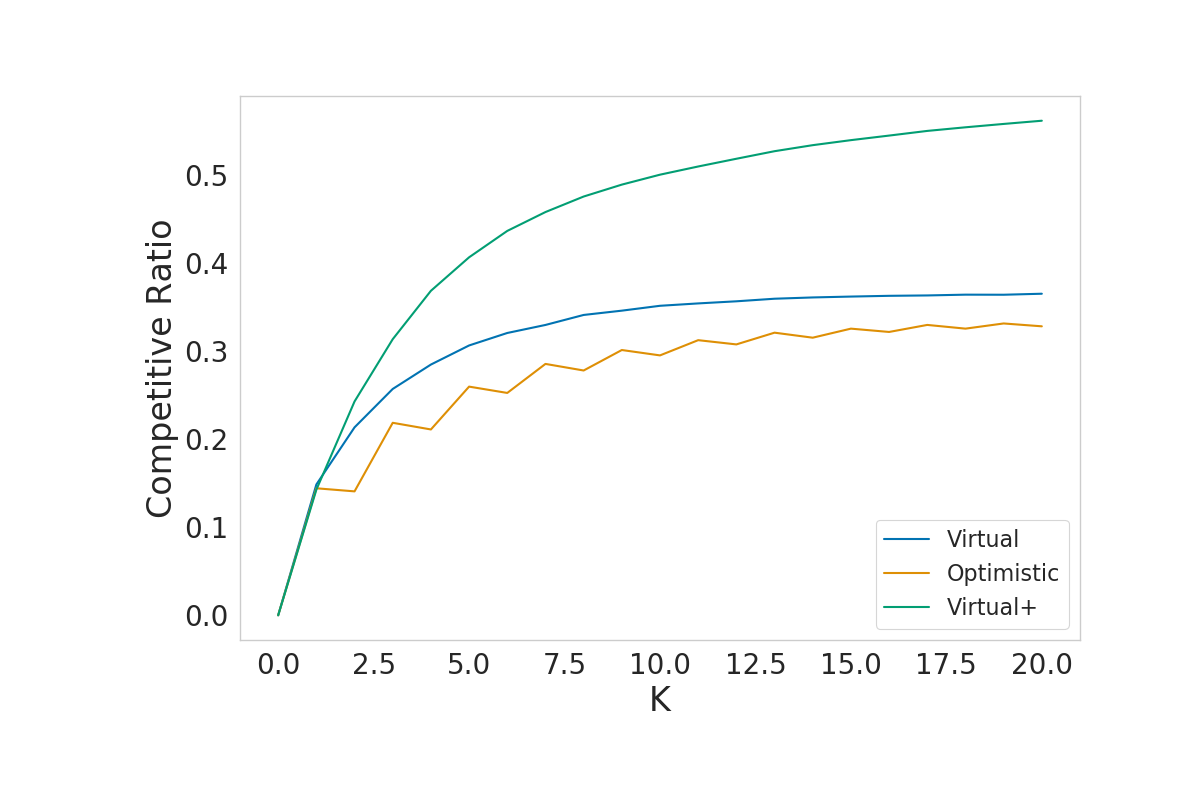
\includegraphics[width=\linewidth]{Figures/Competitive_RatioVar5.png}
    \caption{Virtual+ $k \geq 2$ proof.}
    \label{fig:general_k}
    \vspace{-15pt}
\end{figure}
\begin{proof}
First note that by \citet[Lemma 3.3]{albers2020new} we can show that the competitive ratio for the $k$-secretary problem for a monotone algorithm is equal to 
\begin{equation}
    C = \frac{1}{k}\sum_{a=1}^k \mathbb{P}(i_a \in S_\mathcal{A}), \label{eq:C_as_sum_prob1}
\end{equation}
where $i_a$ is the index of the $a^{th}$ secretary picked by the optimal offline solution ---i.e. $i_a$ is a top-$k$ secretary of $\mathcal{D}$. By Lemma \ref{lemma_monotone} \algoname \ is a monotone algorithm and we may use ~\eqref{eq:C_as_sum_prob1}.

\begin{align}
    \mathbb{P}(i_a \in S_\mathcal{A}) 
    &= \sum_{j=t}^{n-1} \mathbb{P}(i_a \in S_\mathcal{A} \text{ at time-step }j+1) \label{p_picked_equal_not_filled} \\
    &= \frac{1}{n}\sum_{j=t}^{n-1} \mathbb{P}(|S_{\mathcal{A}}| < k \text{ at time-step } j + 1) \notag
\end{align}

Now, we compute $\mathbb{P}(|S_{\mathcal{A}}| < k \text{ at time-step } j+1)$ by decomposing this probability into smaller events  $\mathbb{P}(|S_{\mathcal{A}}| = \nu \text{ at time-step } j+1)$ where $\nu \in [0,\dots,k-1]$.

We may compute the probability of $\mathbb{P}(|S_{\mathcal{A}}| = \nu \text{ at time-step } j+1)$ in the following manner. First, let us consider the scenario where $\nu$ elements are selected by \algoname\ at time steps $p_1$, $p_2, \dots, p_{\nu}$. 
Now, in order for an element to be selected at position $p_\nu$ that element must be one of the top $k$ elements up to time-step $j+1$. Therefore we have a factor $k/j$ in our equation. Now, in order to guarantee that no elements are picked after the position $p_\nu$ we additionally need to ensure that the remaining top-$k$ up to $j+1$ elements appear before $p_\nu$ which results in a factor of ${p_{\nu} - 1 \choose k - 1}/{j-1 \choose k - 1}$. 
Similarly, we may recursively calculate the corresponding factor for each position $p_{\nu-1} \dots p_1$. However, we also need to guarantee that no elements are picked within the time interval $[t+1 \dots p_1-1]$
---i.e. before $p_1$. The probability for this occurring is then ${t \choose k}/{p_1-1 \choose k}$ as this corresponds an ordering where the top-$k$ elements up to $p_1 - 1$ all appear in the sampling phase.
Thus, the probability $p_{t,j}^{k,\nu}:=\mathbb{P}(|S_{\mathcal{A}}| = \nu \text{ at time-step } j+1)$ is :
\begin{align}
    p_{t,j}^{k,\nu}
    &= \sum_{t+1 \leq p_1 < p_2 < \dots <p_{k-1} \leq j}\frac{k}{j} \frac{{p_{\nu} - 1 \choose k-1}}{{j-1 \choose k-1}}\frac{k}{p_{\nu} - 1}
    \frac{{p_{{\nu}-1} - 1 \choose k-1}}{{p_{\nu} - 2 \choose k-1}}\frac{k}{p_{\nu-1} - 1}\dots \frac{k}{p_2 - 1}\frac{{p_1 - 1 \choose k - 1}}{{p_2 - 2 \choose k-1}} \frac{{t \choose k}}{{p_1-1 \choose k}}\\
    & = \frac{t(t-1)\dots(t-k+1)}{j(j-1)\dots (j - k + 1)}\sum_{t+1 \leq p_1 < p_2 < \dots <p_{k-1} \leq j}
    \frac{k^{\nu}}{(p_\nu-k)(p_{\nu-1} - k)\dots(p_1 - k)}
\end{align}

Therefore, the probability of not exceeding $k$-selections, $p_{t,j}^k =\sum_{\nu=0}^{k-1} p_{t,j}^{k,\nu} $, to get before time step $j + 1$ is:
\begin{align}
   \notag
    & \frac{t(t - 1)...(t - k + 1)}{j (j - 1) \dots (j - k + 1)} \bigg(1 + k\hspace{-1em}\sum_{p_1 = t + 1\dots j}^{}\frac{1}{p_1 - k} + \dots
    + {k^{k - 1}}\hspace{-2em}\sum_{\substack{p_1 = t + 1 \dots p_2 - 1  \\\vdots\\ p_{k-1} = t + 1 \dots j}}\frac{1}{(p_1 - k)\dots (p_{k-1} - k)} \bigg)%%\\
    %& = 
    %\frac{t(t - 1)...(t - k + 1)}{j (j - 1) \dots (j - k + 1)} \bigg(1 + k\hspace{-0.5 em}\sum_{p_1 = t + 1}^{j}\frac{1}{p_1 - k} + 
     %\dots  +
     %{k^{k - 1}}\sum_{p_1 = t + 1}^{p_2 -1}\frac{1}{ (p_{1} - k)} \dots \sum_{p_{k-1} = t + 1}^{j}\frac{1}{ (p_{k-1} - k)} \bigg) 
\end{align}
Next, we make use of  
Lemma~\ref{lemma_three}:
\begin{align}
 p_{t,j}^{k} \geq 
     \frac{t(t - 1)\dots (t - k + 1)}{j(j - 1)\dots(j - k + 1)}\left(1 + \frac{k}{1!}\ln \Big(\frac{j - k}{t}\Big) +  \dots + \frac{k^{k - 1}}{(k-1)!}\ln^{k - 1}\Big(\frac{j - k}{t}\Big)\right)
\end{align}
Then we get that the total competitive ratio is: 
\begin{align}
     & \frac{1}{n}\sum_{j = t}^{n - 1}
     \frac{t(t - 1)\dots (t - k + 1)}{j(j - 1)\dots(j - k + 1)}\bigg(1 + \frac{k}{1!}\ln \Big(\frac{j - k}{t}\Big) +  \dots + \frac{k^{k - 1}}{(k-1)!}\ln^{k - 1}\Big(\frac{j - k}{t}\Big)\bigg)\\
     & \geq
     \frac{1}{n}\int_{j = t}^{n}
     \frac{t(t - 1)\dots (t - k + 1)}{j(j - 1)\dots(j - k + 1)}\bigg(1 + \frac{k}{1!}\ln \Big(\frac{j - k}{t}\Big) + \dots + \frac{k^{k - 1}}{(k-1)!}\ln^{k - 1}\Big(\frac{j - k}{t}\Big)\bigg)\\
     & \geq
     \frac{1}{n}\int_{j = t}^{n}
     \frac{t(t - 1)\dots (t - k + 1)}{j^k}\bigg(1 + \frac{k}{1!}\ln \Big(\frac{j - k}{t}\Big) + \dots + \frac{k^{k - 1}}{(k-1)!}\ln^{k - 1}\Big(\frac{j - k}{t}\Big)\bigg)
\end{align}
Now notice that:
\begin{equation}
    \label{identity_two}
    \int\frac{1}{a!} \frac{\ln^a(x)}{x^k} dx = - \frac{1}{x^{k - 1}}\sum_{m = 0}^{a}\frac{1}{m!}(k -1)^{m - 1 -a }\ln^m(x)
\end{equation}
Using the identity in ~\eqref{identity_two} we compute the competitive ratio as:
\begin{align}
     & \geq\frac{t(t - 1)\dots (t - k + 1)}{n}
     \bigg(\sum_{a = 0}^{k - 1}- \frac{1}{j^{k - 1}}{ k ^ a }\sum_{m = 0}^{a}\frac{1}{m!}(k -1)^{m - 1 -a }\ln^m\Big(\frac{j - k}{t}\Big) \bigg) \Big|_{j = t}^{n}\\
     & =
     \frac{t(t - 1)\dots (t - k + 1)}{n}\bigg(- \frac{1}{j^{k - 1}}\sum_{m = 0}^{k - 1}\frac{1}{m!}\Big(\sum_{a = m}^{k - 1}{k ^ a}(k - 1)^{m - a - 1}\Big)\ln^m{\Big(\frac{j - k}{t}\Big)}\bigg)\Big|_{j = t}^{n}
\end{align}
For threshold $t = \alpha n $ where $\alpha \in (0,1)$ and as $n \xrightarrow{}\infty$ our competitive rate becomes:
\begin{align}
    & \alpha \bigg(\sum_{a = 0}^{k - 1}{ k ^ a }{(k - 1)}^{-1 - a}\Big) - \alpha^k\Big(\sum_{m=0}^{k - 1}\frac{1}{m!}\Big(\sum_{a = m}^{k - 1}{ k ^ a }(k - 1)^{m - a - 1}\Big)\ln^m\Big(\frac{1}{\alpha}\Big)\bigg)\\
    & = \alpha\left({\left(\frac{k}{k-1}\right)}^{k} - 1\right) - \alpha^k\left(\sum_{m-0}^{k-1}\left(\frac{\frac{k^k}{(k-1)^{k-m}} - k^m}{m!}\right)(-1)^{m+1}\ln^m(\alpha)\right)
\end{align}
\end{proof}
\begin{definition}
\label{monotone_defn}
An algorithm is called monotone if the probabilities of selecting items $i$ and $j$ satisfy $p_i \geq p_j$ whenever the item values $v_i > v_j$ holds for any two items.
\end{definition}

\begin{lemma}
\label{lemma_monotone}
\algoname \ is a monotone algorithm. 
\end{lemma}
\begin{proof}
    In order to prove that \algoname \ is monotone as defined in Definition \ref{monotone_defn} we must prove that $p_i \geq p_j$ (where $p_i$ is the probability of picking the item $i$) for any two items where $v_i > v_j$. Without loss of generality let us consider a decreasing ordering of $n$-elements based on their values ---i.e. $v_1 > v_{2} > \dots > v_n$. 
    
    
    
    We prove that $p_i \geq p_{i+1}$ for all $i \in [1, \dots, n-1]$ by showing that for each input sequence where $v_{i+1}$ is accepted, there exists a unique input sequence where $v_i$ is accepted. Let us consider a permutation $\pi$ where $v_{i+1}$ appeared and was accepted at time step $a$ while $v_i$ appeared at time step $b$. By swapping $v_i$ and $v_{i+1}$ we obtain a new permutation $\pi'$ where $v_i$ now appears at $a$ and $v_{i+1}$ at $b$. We now study the two following cases.
    
    \xhdr{Case 1: $a < b$}
    
    If $a < b$ notice that the reference set, $R$, and the selected set $S_{\mathcal{A}}$, are exactly the same at time step $a$ for both permutations $\pi$ and $\pi'$. Therefore, if $v_{i+1}$ was accepted at time step $a$ in permutation $\pi$ then $v_i$ will also be accepted at time step $a$ in permutation $\pi'$ since $v_i > v_{i+1}$.   

    \xhdr{Case 2: $a > b$}
    
    If $a > b$ notice that $R$---by definition of \algoname---at time step $a$ contains top-$k$ elements observed in the first $a-1$ time steps. 
    Now the $k$-th element in $R$ at time-step $a$ must satisfy,
    \begin{equation*}
        R^a_{\pi}[k] \geq R^a_{\pi'}[k],
    \end{equation*}
    where $R^a_{[\cdot]}[k]$ corresponds to the $k$-element in the reference set for a specific permutation at time step $a$. Hence, we know that $v_{i} > v_{i+1} \geq R^a_{\pi}[k] \geq R^a_{\pi'}[k]$ as $v_{i+1}$ was assumed to be picked.
    
    
    Furthermore, the $S_{\mathcal{A}}$ and $R$ is the same for permutations $\pi$ and $\pi'$ at time-step $b$. Now by our primary assumption that $v_{i+1}$ is picked at time-step $a>b$ in $\pi$ this means that $v_i$ must be  $v_i \geq R^b_{\pi}[k]$ since $v_i > v_{i+1}$. However, observe that $v_i$ and $R^b_{\pi}[k]$ cannot be consecutive in value as $v_{i+1}$ appears at time-step $a > b$ in permutation $\pi$. This implies that $v_{i+1}$ must also be selected at time step $b$ in permutation $\pi'$ since $v_i$ and $v_{i+1}$ are consecutive in value. By a similar argument based on consecutive order of values between time steps $a$ and $b$ precisely the same elements will be selected in both $\pi$ and $\pi'$. The argument that   $v_{i} > v_{i+1} \geq R^a_{\pi}[k] \geq R^a_{\pi'}[k]$ implies that if $v_{i+1}$ is selected in permutation $\pi$, $v_i$ will also be selected in permutation $\pi'$. The claim then follows by applying the inequality $p_i \geq p_{i+1}$ in an iterative fashion.
\end{proof}
\begin{lemma} 
\label{lemma_three}
Let $f_i \,, \,i = 1 \ldots k$ be decreasing positive functions then we have 
\begin{equation}
    \sum_{p_1=a_1}^{b_1} \ldots \sum_{p_k=a_k}^{p_{k-1}} f_1(p_1) \ldots f_k(p_k)
    \geq \int_{x_1=a_1}^{b_1+1} \ldots \int_{x_k = a_k}^{x_{k-1}+1}  f_1(x_1) \ldots f_k(x_k) dx_1\dots dx_k
\end{equation}
\end{lemma}
\begin{proof}
    The main proof step involves in first noticing that since the functions $f_i \,, \,i = 1 \ldots k$ are decreasing and are positive we have, 
    \begin{equation}
        f_1(p_1) \ldots f_k(p_k) \geq  f_1(p_1) \ldots  f_{k-1}(p_{k-1})\int_{x_k = p_k}^{p_k+1} f_k(x_k) dx_k
    \end{equation}
    Thus, by summing this inequality for $p_k= a_k \ldots p_{k-1}$, we get
    \begin{equation}
    \sum_{p_k=a_k}^{p_{k-1}} f_1(p_1) \ldots f_k(p_k)
    \geq  f_1(p_1) \ldots  f_{k-1}(p_{k-1})  \int_{x_k = a_k}^{p_{k-1}+1} f_k(x_k) dx_k
    \end{equation}
    Now, because the functions $f_i \,, \,i = 1 \ldots k$ are decreasing and positive we have, 
     \begin{align}
    \mathcal{S} 
    &= \sum_{p_k=a_k}^{p_{k-1}} f_1(p_1) \ldots f_k(p_k)\\
    &\geq  f_1(p_1) \ldots  f_{k-2}(p_{k-2})  \int_{x_{k-1} = p_{k-1}}^{p_{k-1}+1} f_{k-1}(x_{k-1})  \int_{x_k = a_k}^{p_{k-1}+1} f_k(x_k) dx_{k-1}dx_k \\
    &\geq f_1(p_1) \ldots  f_{k-2}(p_{k-2})  \int_{x_{k-1} = p_{k-1}}^{p_{k-1}+1} f_{k-1}(x_{k-1})  \int_{x_k = a_k}^{x_{k-1}} f_k(x_k) dx_{k-1}dx_k 
    \end{align}
    where for the last inequality we used the fact that $x_{k-1} \in [p_{k-1}, p_{k-1}+1]$.
    Finally, by summing for $p_{k-1} = a_{k-1} \ldots p_{k-2}$, we get,
    \begin{align}
    \sum_{p_{k-1}=a_{k-1}}^{p_{k-2}}\mathcal{S} &= \sum_{p_{k-1}=a_{k-1}}^{p_{k-2}} \sum_{p_k=a_k}^{p_{k-1}} f_1(p_1) \ldots f_k(p_k)\\
    &\geq f_1(p_1) \ldots  f_{k-2}(p_{k-2})  \int_{x_{k-1} = p_{k-1}}^{p_{k-1}+1} f_{k-1}(x_{k-1})  \int_{x_k = a_k}^{x_{k-1}} f_k(x_k) dx_{k-1}dx_k
    \end{align}
    Using a recursive argument we finally get,
    \begin{equation}
    \sum_{p_1=a_1}^{b_1} \ldots \sum_{p_k=a_k}^{p_{k-1}} f_1(p_1) \ldots f_k(p_k)
    \geq \int_{x_1=a_1}^{b_1+1} \ldots \int_{x_k = a_k}^{x_{k-1}+1}  f_1(x_1) \ldots f_k(x_k) dx_1\dots dx_k
\end{equation}
\end{proof}


\clearpage
\subsection{Analytic computation of $C_k$ for \algoname}

\begin{table}[ht!]
    \centering
    \caption{Values of the Competitive ratio $C_k$ and the associated optimal $\alpha_k$ needed to compute the threshold for \algoname. Note that for $5\leq k\leq 100$ the competitive ratio of \textsc{Single-Ref} provided by~\citet{albers2020new} outperforms \algoname's competitive ratio. However, our analysis provides a tractable way to scale the analytic computation of the competitive ratio with $k$ as the function to optimize (and its gradients) in Theorem~\ref{thm:general_k_theorem1} is $\mathcal{O}(k)$.}
    \vspace{2pt}
    \begin{tabular}{ccccccccccc}
     \toprule
          $k$ & 2 &3 & 4 & 5 & 100 & 200 &300 &400 & 500 & 600\\
         \midrule
        $C_k$ & .4273&.4575&.4769&.4906&.5959&.6062&.6108&.6136&.6156&.6170 \\
        $\alpha_k$ & .3824 &.3867&.3884&.3890&.3781 &.3755 &.3743&.3735&.3729&.3726 \\
        \bottomrule
    \end{tabular}
    \label{tab:C_k}
\end{table}